% Chapter 2

\chapter{Conception et Développement} % Chapter title

\label{ch:2} % For referencing the chapter elsewhere, use \autoref{ch:3} 

La conception et le développement présentés dans ce mémoire s'articulent autour de deux axes principaux. D'une part, nous nous concentrerons sur le modèle \ac{llm}, en suivant toutes les étapes de conception et de développement détaillées dans la section \ref{ch:1:section:ml-process}. Ce processus englobe la collecte initiale des données brutes jusqu'au déploiement final du modèle sélectionné dans un environnement de production. D'autre part, l'attention sera également portée sur le développement du chatbot, qui agit en tant qu'application web. Cette interface utilisateur servira de pont pour accéder au modèle \ac{llm}, facilitant ainsi l'interaction entre les utilisateurs et le système juridique Congolais à travers le chatbot. 

Ce dernier ne représente pas seulement un outil d'accès, mais aussi une manière intuitive et efficace de mettre en application les capacités du modèle \ac{llm}, permettant aux utilisateurs d'obtenir des réponses et des informations juridiques pertinentes de manière interactive.

\section{Les données}

Compte tenu de nos contraintes et objectifs (voir Section~\ref{ch:0:section:limitaions}), les données n'ont pas besoin d'être structurées selon un format particulier, à condition qu'elles soient disponibles sous forme textuelle. Cette flexibilité permet d'exploiter une large variété de sources d'information juridique sans nécessiter de processus de prétraitement complexe pour adapter les données à un format spécifique.

Notre jeu de données sera principalement constitué de documents juridiques provenant de diverses sources officielles et spécialisées, afin d'englober une vaste étendue de la législation et de la doctrine juridique congolaise.

Il est à noter que, bien que les données ne requièrent pas un format spécifique, leur qualité textuelle est essentielle. Cela implique un travail de vérification pour s'assurer de la fiabilité, de la pertinence et de l'actualité des informations collectées. Ce processus permettra de minimiser les erreurs et les ambiguïtés dans les réponses fournies par le chatbot, assurant ainsi une assistance juridique de qualité aux utilisateurs.

\subsection{Les sources d'informations}

\begin{table}[h]
\centering
\begin{tabular}{|l|p{10cm}|}
    \hline
    \textbf{Source} & \textbf{Description} \\
    \hline
    Journal Officiel & Publications officielles qui contiennent les nouvelles lois, décrets, et annonces légales, offrant une source à jour des évolutions législatives. \\
    \hline
    Lois et Décrets & Textes législatifs et réglementaires qui forment la base du système juridique congolais, essentiels pour comprendre le cadre légal en vigueur. \\
    \hline
    Jurisprudences & Décisions de justice issues des tribunaux, fournissant des exemples concrets d’application des lois et des interprétations juridiques. \\
    \hline
    Articles d’Actualité Juridique & Articles publiés par des spécialistes et des médias juridiques, offrant des analyses et des commentaires sur les évolutions récentes du droit et les cas d’intérêt. \\
    \hline
    Doctrine & Contributions d’experts dans le domaine juridique, y compris des analyses détaillées, des critiques, et des interprétations de divers aspects du droit. \\
    \hline
\end{tabular}
\caption{Sources d'information dans le système juridique Congolais}
\label{table:sources-legales-congo}
\end{table}

La numérisation et l'adoption croissante d'Internet en République Démocratique du Congo (RDC) ont considérablement facilité l'accès aux documents légaux officiels. Désormais, un nombre croissant de ces documents est accessible librement en ligne, offrant une opportunité sans précédent pour la recherche et l'analyse juridique. Des plateformes telles que Leganet.cd \footnote{\href{https://leganet.cd}{https://leganet.cd}} jouent un rôle crucial dans l'agrégation et la diffusion de ces documents, constituant ainsi une ressource inestimable pour les praticiens du droit, les chercheurs, et le grand public intéressé par le droit congolais.

Dans ce cadre nous envisageons d'explorer ces diverses sources en ligne. L'objectif est de collecter un large éventail de documents afin de capturer l'étendue et la profondeur du cadre juridique congolais. Cette démarche vise non seulement à fournir à notre modèle une richesse de connaissances et de perspectives sur le droit congolais mais aussi à garantir que les réponses générées soient à la fois informées et pertinentes, reflétant fidèlement les principes et les pratiques juridiques actuels.

Pour faciliter la découverte et l'exploration de ces ressources en ligne, nous envisageons d'utiliser l'\acs{api} Google Custom Search \footnote{\href{https://developers.google.com/custom-search/v1/introduction}{https://developers.google.com/custom-search/v1/introduction}}. Cet outil nous permettra d'automatiser la recherche et de visualiser rapidement les résultats, identifiant ainsi les sites les plus pertinents et fiables où les documents juridiques Congolais sont disponibles. Cette approche automatisée nous aidera à optimiser le processus de collecte de données, en assurant une couverture des sources d'information juridique pertinentes pour notre modèle.

\newpage
\paragraph{Les mots clés} \hspace{0pt}

Les mots-clés jouent un rôle crucial dans le processus de recherche, particulièrement lorsqu'il s'agit de collecter des données spécifiques à un domaine tel que le Droit Congolais. Ils servent de fondement pour affiner les requêtes de recherche et accéder efficacement à l'information pertinente.

\begin{listing}[!ht]
\begin{minted}{python}
keywords = [
    "Constitution", "civil", "Code pénal",
    "Code de travail", "Code foncier ", "Jurisprudence",
    "Droits humains", "Justice transitionnelle", "Droit minier",
    "l'environnement", "commercial", "sociétés",
    "Propriété intellectuelle", "famille", "Violence sexuelle et droit",
    "international humanitaire", "Institutions judiciaires congolaises", 
    "Réforme judiciaire",
    "Lutte contre la corruption", "affaires", "Arbitrage et médiation",
    "bancaire et financier congolais", "fiscal congolais", 
    "Contrats et obligations en congolais",
    "assurances", "santé", "l'éducation",
    "technologies de l'information", "humanitaire",
    "Participation politique et droit"
]
\end{minted}
\caption{Liste des mots clés à utiliser pour la recherche.}
\label{appendix:code:python:search-keywords}
\end{listing}

Cette liste englobe une gamme étendue de domaines juridiques, allant du cadre constitutionnel et législatif général à des domaines plus spécifiques tels que le droit minier, le droit fiscal, et le droit des affaires. Elle inclut également des aspects liés à la jurisprudence, aux publications officielles, et aux analyses d'experts.

Après avoir établi notre liste de mots-clés, nous pouvons créer une fonction qui interagit avec l'\ac{api} Google Custom Search. Cette fonction se sert de la bibliothèque \textbf{Requests} \footnote{\href{https://pypi.org/project/requests/}{https://pypi.org/project/requests/}} pour lancer une requête GET vers l'\acs{url} de l'\acs{api}, en incorporant les paramètres que nous avons spécifiés. Les données renvoyées par l'\acs{api} nous parviennent sous forme de \ac{json}.

\begin{listing}[!ht]
\begin{minted}{python}
params = {
  'q': query,
  'orTerms': ' '.join(keywords).lower(),
  'start': start,
  'key': "xxxxxxxxxxxxxxxxxxxxxxxxxxxxxxxx",
  'cx': 'xxxxxxxxxxxxxxxxxxxx',
  'lr': 'lang_fr',
  'fileType': 'pdf',
  'num': 10
}
\end{minted}
\caption{Dictionnaire des paramètres utile à l'utilisation de l'\acs{api} Google Custom Search}
\label{appendix:code:python:search-google-params}
\end{listing}

Le dictionnaire \textbf{params} contient plusieurs paramètres configurés pour la requête de recherche, des explications détaillées sur l'utilisation des paramètres sont disponible sur la documentation \footnote{\href{https://developers.google.com/custom-search/v1/reference/rest/v1/cse/list}{https://developers.google.com/custom-search/v1/reference/rest/v1/cse/list}} :

\textbf{q}: Le terme principal de la recherche. \\
\textbf{orTerms}: Une chaîne de caractères contenant tous les mots-clés joints par un espace, servant à élargir la recherche à ces termes connexes. \\
\textbf{fileType}: Restreint les résultats aux fichiers d'un type spécifique, ici des \acs{pdf}. \\
\textbf{lr} : Limite la recherche aux documents dans la langue spécifiée, ici le français. \\
\textbf{num}: Détermine le nombre de résultats de recherche à retourner, ici 10 résultats.

La fonction est conçue pour récupérer les résultats d'une seule page à la fois. Pour explorer un ensemble plus large de résultats, nous allons nous appuyer sur la constante \textbf{MAX PAGES}. En procédant à une itération, nous collecterons les résultats de plusieurs pages jusqu'à atteindre la limite fixée par \textbf{MAX PAGES}.

\paragraph{Agrégation des sources} \hspace{0pt}

\begin{listing}[!ht]
\begin{minted}{python}
import requests
import json
import pickle

MAX_PAGES = 10

def search(start=1):
    url = 'https://www.googleapis.com/customsearch/v1'
    query = 'droit congolais'
    response = requests.get(url, params=params)
    return response.json()

try:
    websites = []
    for page in range(1, MAX_PAGES + 1):
        next_page = ((page - 1) * 10) + 1
        results = search(next_page)
        websites.extend(results.get("items", []))

    with open('data.pickle', 'wb') as f:
        pickle.dump(websites, f)
except Exception as e:
    raise e
\end{minted}
\caption{Fonction de recherche via l'\acs{api} Google Custom Search}
\label{appendix:code:python:search-google-function}
\end{listing}

Après avoir recueilli les résultats, nous exploitons la bibliothèque \textbf{Pandas} \footnote{\href{https://pandas.pydata.org/}{https://pandas.pydata.org/}}, qui facilite à la fois la visualisation des données et leur enregistrement dans un fichier au format \ac{csv}.

\begin{listing}[!ht]
\begin{minted}{python}
import pandas as pd 

rows = []
for item in websites:
    row = {
        'Title': item.get('title'),
        'Link': item.get('link'),
        'Snippet': item.get('snippet')
    }
    rows.append(row)

df = pd.DataFrame(rows)
df.head(100)
\end{minted}
\caption{Visualisation et exportation avec Pandas}
\label{appendix:code:python:search-google-visualization}
\end{listing}


\begin{figure}[H]
    \centering
    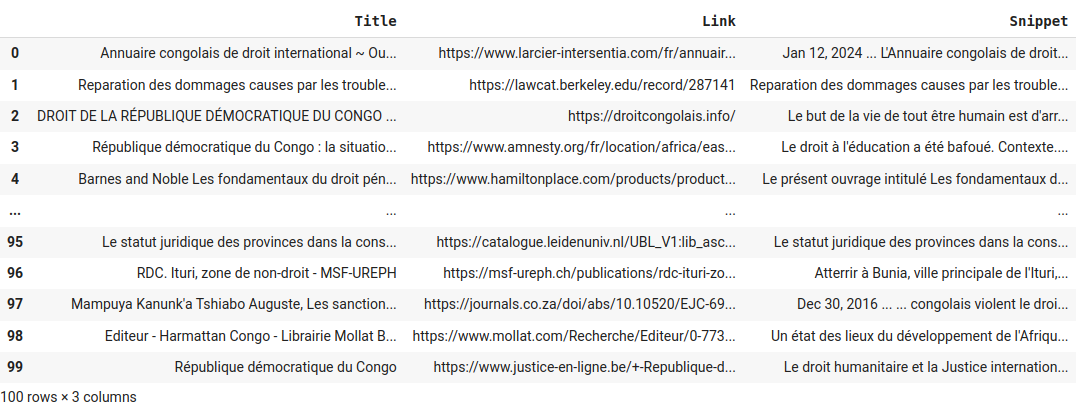
\includegraphics[width=15cm]{gfx/fig-google-search-result.png}
    \caption{Résultat de la recherche via L'\acs{api} Google Custom Search}
    \label{fig:google-search-result}
\end{figure}

Suite à l'emploi de l'\acs{api}, nous avons réussi à récolter plus de 100 résultats distincts, couvrant une variété de sites et de plate-formes dédiés au domaine juridique, et plus spécifiquement au contexte Congolais. Ces résultats nous ouvre la voie vers l'étape suivante de notre processus de collecte de données.

\subsection{Collecte des données}

La collecte de données peut être effectuée via diverses méthodes, dépendant de la nature des données visées et du contexte d'utilisation. Parmi les techniques les plus courantes, on trouve les enquêtes et sondages, l'analyse documentaire, l'observation, et l'exploration de données en ligne. Chacune de ces méthodes a ses propres avantages et inconvénients en termes de coût, de temps, de précision et de couverture des données.

Dans le cadre de notre projet, nous avons opté pour le web scraping comme technique principale de collecte de données. Le web scraping est une méthode d'extraction automatique de données à partir de sites web. Cette technique nous permet de récupérer efficacement un grand volume de documents, en particulier des fichiers \acs{pdf} liés au droit congolais, disponibles sur divers sites et plateformes spécialisés.

Le web scraping repose sur l'utilisation de scripts ou de programmes qui envoient des requêtes aux serveurs web, analysent le \acs{html} de la page pour identifier et extraire les informations nécessaires, et sauvegardent ces informations dans un format structuré pour une utilisation ultérieure. Dans notre cas, cette méthode est particulièrement pertinente pour télécharger automatiquement une multitude de documents juridiques, ce qui constitue une ressource inestimable pour notre base de données \cite{Chakrabarti_2002}.
 
\subsubsection{Conception d'un web crawler}

Un web crawler, également connu sous le nom de web scraper ou spider, est un logiciel conçu pour parcourir automatiquement le \ac{www} en suivant les liens entre les pages web. Il est principalement utilisé pour indexer le contenu des sites web, permettant aux moteurs de recherche de collecter, classer et servir les informations recherchées par les utilisateurs. Le processus implique la visite d'une page web, la lecture de son contenu, l'extraction des liens, puis le suivi de ces liens vers d'autres pages, et ainsi de suite, formant une toile étendue de données recueillies \cite{frwiki:205243717, Chakrabarti_2002, BRIN1998107}.

Le fonctionnement d'un web crawler, tel qu'initialement conceptualisé par Larry Page, repose sur un principe fondamental relativement simple, mais puissant dans sa capacité à organiser l'information sur le web. En substance, le processus peut être décrit par quelques étapes de base codées : le crawler commence par visiter une page web spécifiée, extrait tous les liens présents sur cette page, les enregistre pour un suivi ultérieur, puis répète ce processus de manière récursive pour chaque nouveau lien découvert. Ce mécanisme permet au crawler de naviguer à travers le vaste réseau du web, en cataloguant les ressources trouvées chemin faisant.

\subsubsection{Notre approche}

Dans notre cas, l'objectif s'affine vers une recherche plus ciblée : nous visons spécifiquement à localiser et récupérer des documents au format \ac{pdf}. Ce choix implique une adaptation du processus de crawl standard pour filtrer les liens et ne retenir que ceux qui mènent directement à des fichiers \ac{pdf}. En d'autres termes, notre crawler est conçu pour non seulement suivre les liens, mais aussi pour identifier et sauvegarder les chemins vers des documents \ac{pdf}, en ignorant les autres types de fichiers ou de contenu web. Cette spécialisation permet une collecte de données plus efficace et pertinente pour nos besoins de recherche juridique, garantissant que seuls les documents correspondant à nos critères soient téléchargés et stockés pour une analyse ultérieure.

\begin{figure}[H]
    \centering
    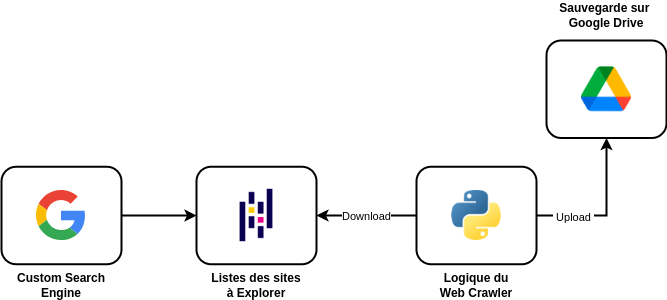
\includegraphics[width=12 cm]{gfx/fig-crawler-architecture.png}
    \caption{Architecture du web crawler [le nôtre]}
    \label{fig:crawler-architecture}
\end{figure}

Comme illustré dans la figure~\ref{fig:crawler-architecture}, notre méthodologie s'aligne étroitement sur le modèle éprouvé par l'architecture de Google \cite{BRIN1998107}. Le point d'entrée de notre processus est l'utilisation de l'API Google Custom Search pour générer un inventaire de sites web spécialisés dans le droit congolais. Cette première récolte de données est ensuite convertie en un DataFrame \footnote{\href{https://pandas.pydata.org/docs/reference/api/pandas.DataFrame.html}{https://pandas.pydata.org/docs/reference/api/pandas.DataFrame.html}} Pandas, ce qui facilite la visualisation et le filtrage des données pour affiner notre recherche. Après avoir épuré cette liste, un script Python prend le relais, parcourant méthodiquement les sites pour y télécharger les fichiers \ac{pdf} disponibles. Enfin, dans la dernière étape de notre flux de travail, les \ac{pdf} ainsi collectés sont stockés sur Google Drive \footnote{\href{https://developers.google.com/drive/api/guides/about-sdk}{https://developers.google.com/drive/api/guides/about-sdk}}, assurant leur sauvegarde dans le cloud et permettant un accès aisé pour des analyses futures.

\paragraph{Implémentation itérative} \hspace{0pt}

\begin{listing}[!ht]
\begin{minted}{python}
import requests
from bs4 import BeautifulSoup

def crawl_link(url, from_root = False):
    response = requests.get(url)
    soup = BeautifulSoup(response.content, 'html.parser')
    links = soup.find_all('a', href=True)

    for link in links:
        href = link.get('href')
        if from_root:
            base = urlparse(url)
            href = f'{url}{href}'
        if href and href.endswith('.pdf'):
            download_pdf(href, DOWNLOAD_PATH)
            print(f'Downloaded {href}')
\end{minted}
\caption{Implémention itérative du crawler}
\label{appendix:code:python:iterative-crawl-function}
\end{listing}

Le script (implémentation itérative) principal de notre crawler est bâti sur l'usage de deux puissantes bibliothèques Python : requests et BeautifulSoup \footnote{\href{https://pypi.org/project/beautifulsoup4/}{https://pypi.org/project/beautifulsoup4/}}. requests  est la porte d'entrée pour accéder aux contenus des sites web en récupérant leur code \ac{html}.

Une fois le contenu \ac{html} obtenu, c'est là qu'intervient \textbf{BeautifulSoup}, une bibliothèque qui se distingue par sa capacité à analyser et à extraire des informations à partir de documents \ac{html} et \ac{xml}. Grâce à BeautifulSoup, nous pouvons naviguer dans la structure de la page web, parcourir les différents éléments du \ac{dom}, et extraire précisément les données qui nous intéressent. Elle offre une variété de méthodes pour filtrer les éléments de la page, tels que les liens, en fonction de leur balisage et de leurs attributs \cite{frwiki:203869267}.

Dans la pratique, notre script exploite BeautifulSoup pour identifier spécifiquement les liens de téléchargement de fichiers \ac{pdf}. Nous pouvons isoler ces éléments grâce à leurs attributs distinctifs (par exemple, href se terminant par .pdf) et récupérer les \acs{url}s nécessaires pour lancer le téléchargement.

\paragraph{Téléchargements des fichiers} \hspace{0pt}

L'automatisation du téléchargement d'un volume conséquent de fichiers présente le risque inhérent de doublons, ce qui pourrait entraver l'efficacité de notre base de données et compliquer les analyses futures. Pour pallier ce problème et garantir l'unicité de chaque document, nous avons recours à une stratégie de renommage judicieuse : attribuer à chaque fichier un nom basé sur un hachage \ac{md5} \footnote{"\ac{md5} est une fonction de hachage cryptographique qui calcule, à partir d'un fichier numérique, son empreinte numérique (en l'occurrence une séquence de 128 bits ou 32 caractères en notation hexadécimale) avec une probabilité très forte que deux fichiers différents donnent deux empreintes différentes." \cite{frwiki:203545836}} de son contenu.

\begin{listing}[!ht]
\begin{minted}{python}
import os
import hashlib

def calculate_md5(file_path):
    hash_md5 = hashlib.md5()
    with open(file_path, 'rb') as f:
        for chunk in iter(lambda: f.read(4096), b""):
            hash_md5.update(chunk)
    return hash_md5.hexdigest()
\end{minted}
\caption{Fonction de hashage \ac{md5} des fichiers}
\label{appendix:code:python:md5-hashing}
\end{listing}

Même un changement minime dans le document entraînera la création d'un hachage radicalement différent. Par conséquent, si deux fichiers distincts portent le même nom mais ont des contenus différents, leur hachage \ac{md5} révélera leur individualité. À l'inverse, si deux fichiers de noms différents présentent un contenu identique, ils seront assignés au même hachage \ac{md5}, ce qui nous permet de détecter et de gérer les doublons \cite{rfc1321}.

En renommant chaque fichier téléchargé avec son hachage \ac{md5}, nous établissons un système de dénomination unique et invariant, indépendant des noms de fichier originaux qui peuvent être arbitraires ou redondants. Cette méthode de renommage par hachage assure donc que chaque fichier dans notre collection est véritablement distinct et facilite l'organisation et la recherche dans la base de données, en éliminant les redondances et en optimisant l'espace de stockage.

\begin{listing}[!ht]
\begin{minted}{python}
import requests
import os
from urllib.parse import urlparse

def download_pdf(url, path):
    try:
        response = requests.get(url, stream=True)
        response.raise_for_status()
        filename = os.path.join(path, os.path.basename(urlparse(url).path))
        
        with open(filename, 'wb') as pdf_file:
            for chunk in response.iter_content(chunk_size=8192):
                pdf_file.write(chunk)
        
        hash = calculate_md5(filename)
        hashedfile = os.path.join(path, hash + '.pdf')
        os.rename(filename, hashedfile)
        print(f'Fichier téléchargé {filename} => {hashedfile}')
    except Exception as e:
        print(f'Erreur lors du téléchargement de {url}: {e}')
\end{minted}
\caption{Fonction de téléchargement des fichiers}
\label{appendix:code:python:md5-hashing}
\end{listing}

Avec une stratégie de nommage optimisée désormais en place, nous sommes en mesure de procéder au téléchargement des fichiers en toute confiance, en alimentant simplement notre fonction avec l'\ac{url} correspondante. Nous exploitons l'environnement Google Colab \footnote{\href{https://colab.research.google.com}{https://colab.research.google.com/}} pour mener à bien ces opérations, bénéficiant de ses capacités de calcul et de sa compatibilité avec d'autres services Google. L'un des avantages notables de Colab est sa capacité à intégrer un disque virtuel Google Drive \footnote{\href{https://colab.research.google.com/notebooks/io.ipynb}{https://colab.research.google.com/notebooks/io.ipynb}}, que nous pouvons monter et utiliser comme s'il s'agissait d'un répertoire local.

Les fichiers téléchargés peuvent être directement enregistrés sur le Drive monté sans nécessiter de transferts ultérieurs, permettant ainsi un accès immédiat et une organisation structurée. En utilisant le système de fichiers virtuel de Google Drive, nous simplifions considérablement le processus de sauvegarde et de partage des documents, tout en tirant parti de la robustesse et de la redondance des infrastructures de stockage cloud de Google.

\begin{figure}[H]
    \centering
    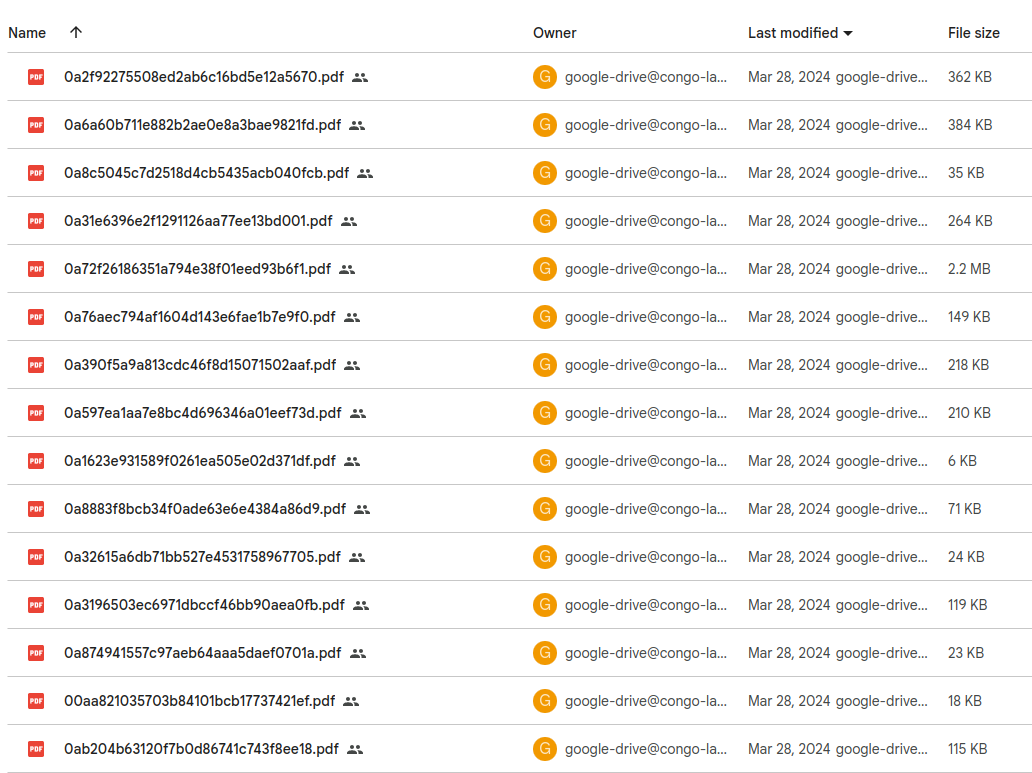
\includegraphics[width=15cm]{gfx/fig-google-drive.png}
    \caption{Documents sur Google Drive après téléchargement}
    \label{fig:crawler-architecture}
\end{figure}

\paragraph{Implémentation Récursive} \hspace{0pt}

Avec l'ajout d'une implémention récursive à notre arsenal, notre crawler transcende les limitations précédentes et s'aventure désormais au-delà d'une page unique. Cette version avancée de notre crawler dispose désormais de la capacité de naviguer méthodiquement à travers un site entier, identifiant et téléchargeant non seulement les documents disponibles sur l'\ac{url} de départ mais aussi en suivant les liens vers d'autres pages pour récupérer les fichiers \ac{pdf} associés.

\begin{listing}[!ht]
\begin{minted}{python}
from urllib.parse import urljoin, urlparse, urlunparse
from urllib.request import urlretrieve

def remove_fragment(url):
        parsed_url = urlparse(url)
        clean_parsed_url = parsed_url._replace(fragment="")
        return urlunparse(clean_parsed_url)
\end{minted}
\caption{Fonction de nettoyage d'\ac{url}}
\label{appendix:code:python:remove-fragment}
\end{listing}

 Le processus débute avec la fonction $remove\_fragment$, qui purifie l'\ac{url} de toute portion inutile, permettant ainsi de concentrer le crawl sur les contenus essentiels des pages. Puis, $recursive\_crawl$ prend le relais, visitant chaque \ac{url} unique seulement une fois grâce à l'ensemble $visited\_urls$ qui assure une trace des pages déjà explorées et prévient les boucles infinies.

Lorsqu'une page est visitée, toute \ac{url} se terminant par $.pdf$ est immédiatement transmise à $download_pdf$, qui procède au téléchargement du fichier et le sauvegarde dans un emplacement spécifique sur Google Drive. Tous les autres liens sont examinés et suivis s'ils appartiennent au même domaine que l'\ac{url} de départ, et ce processus se poursuit de façon récursive. C'est une exploration en profondeur, déployant une toile d'araignée qui s'étend sur l'intégralité du site.

\begin{listing}[!ht]
\begin{minted}{python}
def recursive_crawl(start_url, url, visited_urls):
        url = remove_fragment(url)
        if url in visited_urls:
            return

        visited_urls.add(url)
        print(url)

        try:
            response = requests.get(url)
            response.raise_for_status()
            soup = BeautifulSoup(response.text, 'html.parser')

            if url.lower().endswith('.pdf'):
                download_pdf(url, '/content/drive/MyDrive/DATA/LawLLM/PDF/')
                print(f"File-Downloaded: {url}")

            for link in soup.find_all('a', href=True):
                href = link['href']

                if not urlparse(href).scheme:
                    next_url = urljoin(url, href)
                    recursive_crawl(start_url, next_url, visited_urls)

                elif urlparse(href).hostname == urlparse(start_url).hostname:
                    recursive_crawl(start_url, href, visited_urls)

        except Exception as e:
            print(f"Error while processing {url}: {e}")

def recursive_crawl_link(start_url, destination):
    visited_urls = set()
    recursive_crawl(start_url, start_url, visited_urls)
\end{minted}
\caption{Implémentation récursive du crawler}
\label{appendix:code:python:remove-fragment}
\end{listing}

Cela transforme notre crawler en un outil dynamique et exhaustif, capable d'extraire méthodiquement une richesse d'informations et de ressources souvent enfouies dans la structure des sites web. En exploitant $recursive\_crawl$, nous pouvons cartographier un domaine entier, saisissant non seulement la superficie mais aussi plongeant dans les couches les plus profondes de contenu.

L'implémentation récursive signifie également que notre crawler peut fonctionner avec une autonomie et une efficacité élevées, nécessitant une supervision minimale et permettant aux chercheurs et aux professionnels de se concentrer sur l'analyse et l'exploitation des données collectées plutôt que sur le processus de collecte lui-même.

Cette méthode enrichit considérablement notre ensemble de données, non seulement en volume mais aussi en variété, fournissant une image complète et nuancée du domaine juridique congolais, qui est notre objectif premier. Elle souligne l'efficacité de la programmation récursive dans des applications pratiques telles que le web scraping, démontrant comment une approche algorithmique bien pensée peut considérablement simplifier des tâches autrement ardues et complexes.

\begin{figure}[H]
    \centering
    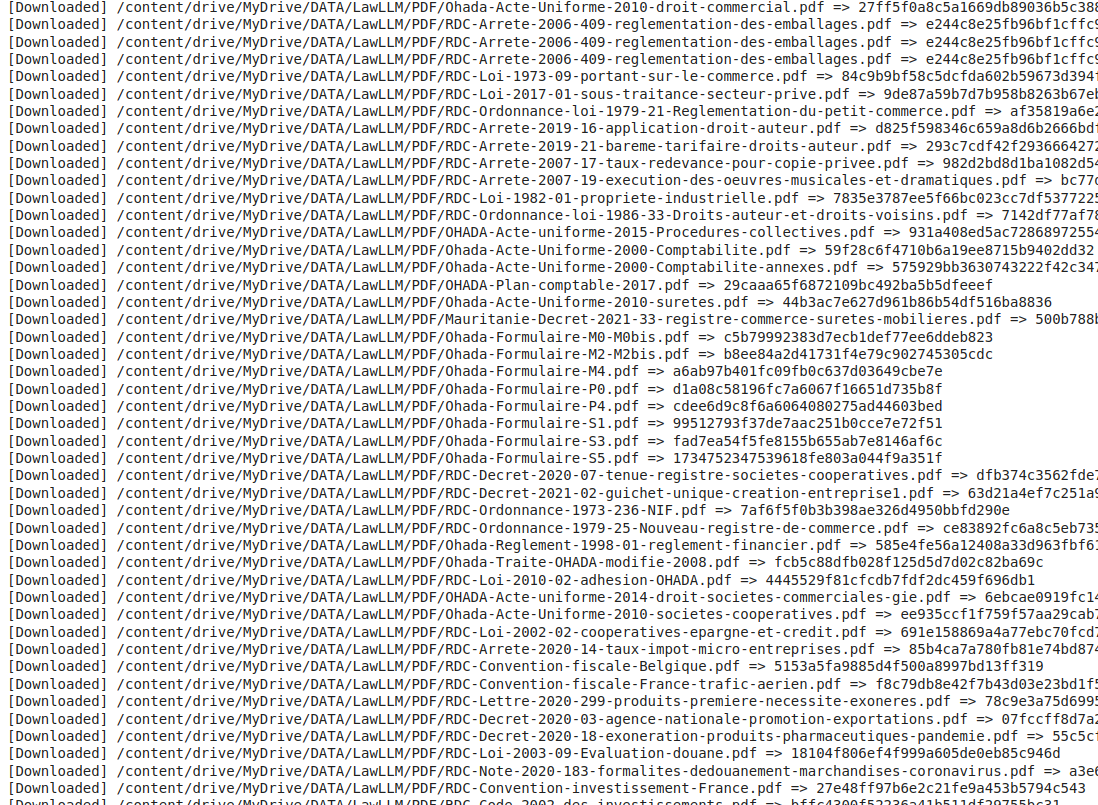
\includegraphics[width=15cm]{gfx/fig-crawler-downloading.png}
    \caption{Téléchargement en cours, approche itérative}
    \label{fig:crawler-downloading}
\end{figure}

\begin{figure}[H]
    \centering
    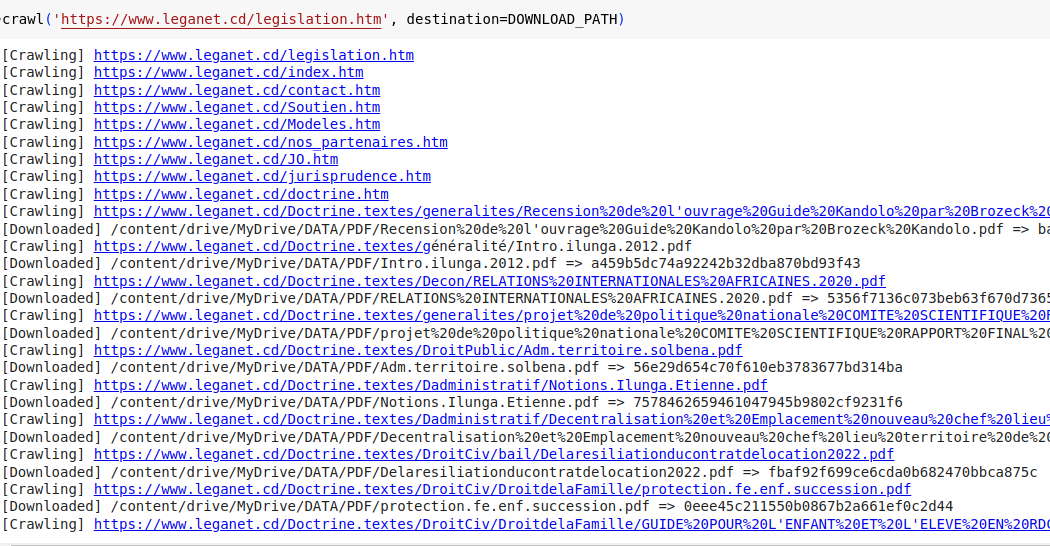
\includegraphics[width=15cm]{gfx/fig-download-recursive.png}
    \caption{Téléchargement en cours, approche récursive}
    \label{fig:crawler-downloading}
\end{figure}

\subsection{Pré-traitement et Formalisations des données}

Après avoir mené à bien le téléchargement de plus de 4000 documents, il est essentiel de reconnaître que bien que ces fichiers soient une mine d'informations, leur forme brute n'est pas directement utilisable. Par conséquent, l'étape de pré-traitement devient cruciale. Dans notre contexte, le pré-traitement consiste principalement à convertir le contenu de ces documents \acs{pdf} en texte exploitable.

Le processus d'extraction de texte des PDF est un défi en soi, car il implique de décoder les diverses manières dont le contenu est encapsulé dans un document \acs{pdf}. Cela peut inclure la gestion de la mise en page complexe, l'extraction de texte à partir d'images incorporées par \ac{ocr} et la préservation de la structure sémantique des informations.

\paragraph{Extraction du texte} \hspace{0pt}

L'extraction de texte à partir de documents PDF est une opération qui peut être réalisée avec efficacité en utilisant la bibliothèque Fitz, également connue sous le nom de PyMuPDF \footnote{\href{https://pymupdf.readthedocs.io/en/latest/}{https://pymupdf.readthedocs.io/en/latest/}}.

\begin{listing}[!ht]
\begin{minted}{python}
def extract_text(pdf_path):
    doc = fitz.open(pdf_path)
    text_content = []

    for page_num in range(len(doc)):
        page = doc.load_page(page_num)
        text = page.get_text("text")
        text_content.append({
            'page': page_num + 1, 
            'type': 'text', 
            'content': text
        })

        # extract text in image

    doc.close()
    return text_content
\end{minted}
\caption{Extraction du contenu d'un document PDF}
\label{appendix:code:python:remove-fragment}
\end{listing}

\paragraph{Extraction du texte sur image} \hspace{0pt}

Pour extraire du texte à partir d'images, telles que des documents scannés ou numérisés, nous faisons appel à Tesseract. Tesseract est un moteur d'\ac{ocr} open source, considéré comme l'un des plus précis disponibles. L'\ac{ocr} est une technologie qui permet de convertir différents types de documents, tels que des images numérisées de texte imprimé, des captures d'écran ou des images contenant du texte, en données de texte modifiables et recherchables (voir Code~\ref{appendix:code:python:text-extract-images}) \cite{smith_tesseract_2007}.


\section{Du texte à la création d'Embeddings}

Dans le domaine de l'\ac{ia}, et plus particulièrement dans celui des \ac{llm}, la compréhension directe du texte en langage naturel par un modèle est "\textbf{impossible}". Au lieu de cela, le texte doit être converti en une forme que le modèle peut traiter : une représentation mathématique. Ce processus est essentiel pour que les modèles apprennent et génèrent du langage humain de manière efficace \cite{Embeddings}.

\subsection{La tokenisation}
\label{ch:2:section:tokenization}

Le premier pas vers la transformation du texte en données compréhensibles par une machine est la tokenisation. Ce processus consiste à découper le texte en morceaux plus petits, appelés tokens, qui peuvent être des mots, des phrases, ou même des parties de mots. Ces tokens servent de base pour la construction des représentations numériques.

\begin{figure}[H]
    \centering
    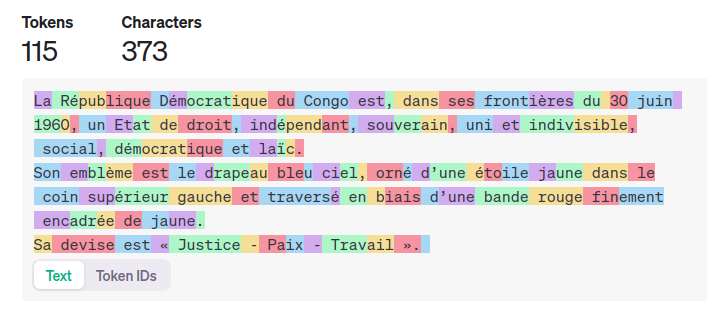
\includegraphics[width=15cm]{gfx/fig-tokenization.png}
    
    \caption{Exemple de tokenisation avec Open AI tokenizer.}
    \label{fig:token}
\end{figure}

\subsection{les Embeddings}
\label{ch:2:section:embeddings}

Après la tokenisation, l'ensemble de tokens sont convertis en un vecteur via un processus appelé embedding. Les embeddings sont des représentations vectorielles denses de mots dans un espace continu de dimensions réduites, par rapport au vocabulaire total. Ces vecteurs capturent non seulement l'identité des mots mais aussi les aspects sémantiques et syntaxiques de ceux-ci, ce qui permet au modèle d'établir des liens entre les mots en fonction de leur contexte et de leur usage (voir section~\ref{ch:1:section:embeddings}).

\begin{figure}[H]
    \centering
    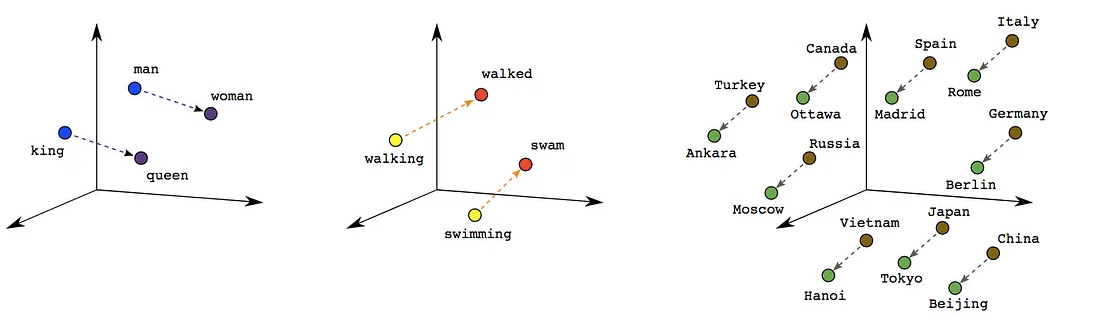
\includegraphics[width=15cm]{gfx/fig-embeddings.png}
    \caption{Représentation vectorielle d'un texte \cite{Anala_2020}}
    \label{fig:crawler-downloading}
\end{figure}

\newpage
\paragraph{Méthodes d'embeddings} \hspace{0pt}

\begin{table}[h]
\centering
\begin{tabular}{|p{3cm}|p{11cm}|}
\hline
\textbf{Méthode} & \textbf{Description} \\ \hline

One-hot Encoding & Chaque mot du vocabulaire est représenté par un vecteur où un seul élément est "1" et tous les autres sont "0". Cette méthode est simple mais inefficace pour les grands vocabulaires et ne capture pas les relations sémantiques \cite{onehotencoding}. \\ \hline
Word2Vec & Développé par Google, Word2Vec utilise un réseau de neurones pour apprendre des vecteurs de mots à partir de grands ensembles de données textuelles. Il existe deux architectures pour Word2Vec : Skip-gram et CBOW (Continuous Bag of Words). Word2Vec est efficace pour capturer les contextes des mots et les relations sémantiques entre eux \cite{mikolov2013efficient}. \\ \hline

GloVe & Une autre méthode populaire qui combine les avantages de la factorisation de la matrice des co-occurrences de mots et des méthodes contextuelles comme Word2Vec. GloVe est particulièrement bon pour saisir des relations subtiles entre les mots \cite{pennington2014glove}. \\ \hline

FastText & Proposé par Facebook, FastText étend Word2Vec pour considérer non seulement les mots mais aussi les séquences de caractères, ce qui le rend efficace pour gérer les mots rares ou mal orthographiés \cite{bojanowski2016enriching}. \\ \hline

Transformers et BERT & Plus récemment, les modèles basés sur l'architecture Transformer, tels que BERT (Bidirectional Encoder Representations from Transformers), utilisent des embeddings contextuels, où la représentation d'un mot peut changer en fonction des mots qui l'entourent dans une phrase. Cela permet une compréhension plus nuancée et dynamique du texte \cite{devlin2018bert}. \\ \hline
\end{tabular}

\caption{Comparaison des méthodes d'embedding de mots}
\label{table:word_embedding_methods}
\end{table}

Il est important de noter que la qualité des embeddings a un impact direct sur la performance du modèle, rendant leur choix et leur implémentation des aspects critiques de la conception des systèmes de \ac{nlp}. 

Il est également essentiel de souligner que la dimension du vecteur généré en fonction des données joue un rôle significatif. En effet, plus la dimension du vecteur est grande, plus il est capable de capturer des nuances fines et complexes du langage. Cependant, il faut également prendre en compte que des vecteurs de plus grandes dimensions requièrent plus de temps pour être générés et peuvent augmenter considérablement la charge computationnelle lors du traitement des données.

\newpage

\begin{table}[h]
\centering
\begin{tabular}{|p{7cm}|p{3cm}|p{3cm}|}
\hline
\textbf{Modèle}            & \textbf{Dimension} & \textbf{Disponibilité} \\ \hline
Mistral-embed              & 1024               & API payante            \\ \hline
text-embedding-3-small     & 1536               & API payante            \\ \hline
text-embedding-3-large     & 3072               & API payante            \\ \hline
voyage-2                   & 1024               & API payante            \\ \hline
Ollama embedding           & 1024               & Gratuit     \\ \hline
\end{tabular}

\caption{Comparatif des modèles d'embedding disponibles}
\label{table:embedding_models}
\end{table}


Dans ce mémoire, nous avons opté pour des embeddings de dimension \textbf{1024}. Ce choix est stratégiquement motivé par deux facteurs clés : 
\begin{itemize}
    \item Premièrement, cette dimension offre une flexibilité optimale en termes d'interchangeabilité des modèles générant lesdits embeddings, permettant ainsi une intégration aisée de diverses technologies d'embedding sans compromettre la compatibilité ou la performance.

    \item Deuxièmement, en considérant les ressources financières à notre disposition, la dimension de 1024 est suffisamment large pour capturer une quantité significative de nuances sémantiques tout en restant gérable d'un point de vue computationnel, ce qui est crucial pour limiter les coûts liés à la puissance de calcul et au stockage.
\end{itemize}

Les différents modèles d'embedding imposent généralement une limite sur la taille du texte pouvant être traité en une seule fois, souvent désignée comme la limite de contexte. Pour contourner cette contrainte et optimiser le traitement des données, nous adopterons une approche où tous nos documents seront subdivisés en segments de 500 caractères chacun. Cette méthode de segmentation nous permet de gérer efficacement les limitations de taille d'entrée tout en préservant le contexte nécessaire à une analyse sémantique significative.

Une fois ces segments générés, nous procéderons à leur embedding avant de les stocker dans une base de données PostgreSQL \footnote{\href{https://www.postgresql.org/}{https://www.postgresql.org/}}. Cette base de données sera configurée avec l'extension "pgvector" \footnote{\href{https://github.com/pgvector/pgvector}{https://github.com/pgvector/pgvector}}, spécialement conçue pour supporter les types de données vectorielles. L'utilisation de PostgreSQL, combinée avec cette extension, nous offre une solution robuste et performante pour la gestion de grands volumes de données vectorielles.

\newpage
\section{\acf{rag}}

De prime abord, il est important de souligner que la création d'un \ac{llm} est un processus coûteux et exigeant en termes de données. Les modèles de langage existants, tels que GPT-4 \cite{openai2023gpt4}, ont été développés avec une quantité massive de données et une puissance de calcul considérable. Cependant, pour adapter ces modèles au contexte juridique congolais, il serait peu pratique, voire impossible, de construire un \ac{llm} à partir de zéro en raison de contraintes de ressources.

Inspiré par Heydar Soudani \cite{soudani2024fine}, notre approche consiste à utiliser un modèle de langage existant comme point de départ (voir Table~\ref{table:llm-models}). En prenant un modèle pré-entraîné, nous pouvons bénéficier des connaissances et des capacités linguistiques déjà intégrées dans le modèle. Nous chercherons ensuite à affiner ce modèle pré-entraîné pour le rendre spécifique au système juridique congolais. 

l'approche du \ac{rag}, combine la génération de texte avec des techniques de recherche d'informations. Le \ac{rag} permet au chatbot d'accéder à une base de connaissances juridiques étendue et de récupérer des informations pertinentes en réponse aux requêtes des utilisateurs. En utilisant des index de recherche efficaces et des algorithmes de récupération d'informations, le chatbot peut fournir des réponses bien informées en s'appuyant sur une grande variété de sources \cite{lewis2021retrievalaugmented}.

\begin{figure}[H]
    \centering
    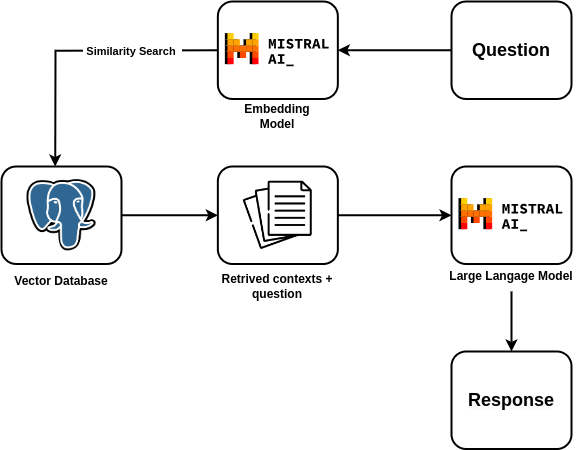
\includegraphics[width=12cm]{gfx/fig-rag-architecture.png}
    \caption{Architecture d'un système \ac{rag} inspiré par \cite{rag_architecture}}.
    \label{fig:rag-architecture}
\end{figure}

L'illustration ci-dessus présente l'architecture de notre approche adaptée pour améliorer la pertinence et la précision des réponses générées par un \ac{llm} dans le domaine juridique congolais.

Le processus débute lorsqu'une question est posée par l'utilisateur, cette question sert de point de départ pour l'ensemble du pipeline :

\subsection{Le modèle d'embedding}
La question est d'abord transformée en une représentation vectorielle à l'aide d'un modèle d'embedding (voir Table~\ref{table:embedding_models}). L'embedding de la question est ensuite utilisé pour effectuer une recherche par similarité dans une base de données vectorielle. 

\subsection{Base de données vectorielle (Vector Store)}
\label{ch:2:section:vector-store}

Cette base de données, alimentée par \textit{PostgreSQL} et l'extension \textit{pgvector}, contient des embeddings de documents récoltés précédemment.

\begin{figure}[H]
    \centering
    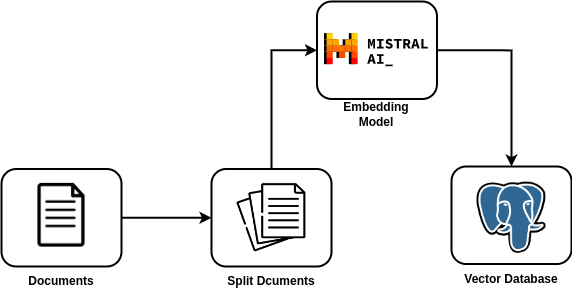
\includegraphics[width=12cm]{gfx/fig-knowledge-base.png}
    \caption{Création de la base de connaissance}.
    \label{fig:knowledge-base}
\end{figure}

Les documents initiaux sont divisés en segments plus petits. Cette segmentation facilite le traitement et l'analyse des textes en morceaux gérables, ici en sous-parties de 500 caractères et chaque segment de texte résultant de la division est ensuite envoyé à un modèle d'embedding et enfin stocké. 

Pour mesurer la similarité entre l'embedding de la question et les embeddings des documents stockés, diverses fonctions de recherche de similarité peuvent être employées. Parmi celles-ci, les plus couramment utilisées sont :

\begin{itemize}
    \item[<->] \textbf{Distance Euclidienne (L2)  : } 
    La distance euclidienne est une mesure de la distance directe entre deux points dans un espace vectoriel.
    
    \item[<\#>] \textbf{Produit Scalaire  :} 
    Le produit scalaire mesure la similarité en calculant la somme des produits des composantes correspondantes de deux vecteurs.
    
    \item[<=>] \textbf{Distance Cosinus :}
    La distance cosinus mesure la similarité entre deux vecteurs en calculant le cosinus de l'angle entre eux.
    
    \item[<+>] \textbf{Distance de Manhattan (L1) :}
    La distance L1, également connue sous le nom de distance de Manhattan, mesure la somme des valeurs absolues des différences entre les composantes correspondantes de deux vecteurs.
\end{itemize}

Par exemple nous pouvons récupérer le contenu des 5 documents les plus proches de la question de l'utilisateur avec les requêtes \ac{sql} suivantes : 

\hspace{1pt}
\begin{listing}[!ht]
\begin{minted}{sql}
SELECT * FROM documents ORDER BY embedding <-> '[3,1,2]' LIMIT 5;
SELECT * FROM documents ORDER BY (embedding <#> '[3,1,2]') * -1 LIMIT 5;
SELECT * FROM documents ORDER BY 1 - (embedding <=> '[3,1,2]') LIMIT 5;
\end{minted}
\caption{Exemple de requêtes \ac{sql} sur les distances entre vecteurs}
\label{appendix:code:sql:embeddings-distances}
\end{listing}

\subsection{Le contexte}

\begin{listing}[!ht]
\begin{minted}{php}
public string $systemMessageTemplate = <<<TEMPLATE
    Ton nom est Juro crée par Bernard Ngandu, 
    Tu es un expert en Droit Congolais (RDC), ton objectif est de vulgariser 
    le droit congolais et de répondre aux questions en utilisant 
    les éléments de CONTEXT suivants. si aucun CONTEXT ne t'es fourni, 
    précise que tu ne peux pas répondre directement à la question

    CONTEXT : {context}
TEMPLATE;
\end{minted}
\caption{Le message système}
\label{appendix:code:php:system-message-template}
\end{listing}

Une fois que des documents pertinents ont été trouvés, ils permettent de créer un contexte riche et informatif. Ce contexte contient tous les éléments nécessaires pour répondre précisément à la question de l'utilisateur et joue un rôle crucial dans la direction que prendra la génération de la réponse par le \ac{llm}.

Pour guider le \ac{llm} de manière efficace, nous utiliserons un message système. Ce message contient des instructions spécifiques que le \ac{llm} devra suivre pour générer une réponse. il sert de cadre et de guide, assurant que le modèle comprend bien la nature de la question, les attentes en termes de format et de contenu de la réponse, et les aspects spécifiques du contexte qui doivent être pris en compte.


\newpage
\section{Conception de l'application Web}

\begin{figure}[H]
    \centering
    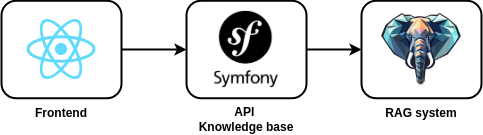
\includegraphics[width=12cm]{gfx/fig-juro-architecture.png}
    \caption{Architecture du chatbot}.
    \label{fig:juro-architecture}
\end{figure}

Maintenant que nous avons les données et l'architecture \ac{rag} en place, nous allons aborder la conception et le développement du chatbot. Ce chatbot est constitué de trois principaux composants : un frontend, une \ac{api}, et le système \ac{rag}. Dans cette section, nous détaillerons le frontend et l'\ac{api}, ainsi que leur interaction avec le système \ac{rag}, nous choissons le nom "Juro" pour notre chatbot, inspiré de la contraction "Juridique" et "Robot".

\subsection{Le frontend}

Le frontend de notre application est développé en utilisant React \footnote{\href{https://fr.react.dev/}{https://fr.react.dev/}}, une bibliothèque JavaScript populaire pour la construction d'interfaces utilisateur dynamiques et réactives. Le frontend sert de point de contact principal pour les utilisateurs, leur permettant de poser des questions et de recevoir des réponses de manière intuitive et conviviale

\paragraph{Les fonctionnalités} \hspace{0pt}

\begin{table}[h]
\centering
\begin{tabular}{|p{12cm}|l|}
\hline
\textbf{Fonctionnalité} & \textbf{Importance} \\ \hline
S'inscrire              & Haute               \\ \hline
S'authentifier          & Haute               \\ \hline
Créer un nouveau chat   & Haute               \\ \hline
Consulter les chats     & Moyenne             \\ \hline
Envoyer un message      & Haute               \\ \hline
Renommer un chat        & Faible              \\ \hline
Supprimer un chat       & Moyenne             \\ \hline
Choisir un chat proposé & Moyenne             \\ \hline
\end{tabular}
\caption{Cas d'utilisation et leur importance}
\label{tab:use_cases}
\end{table}

Les fonctionnalités critiques pour le fonctionnement de base du système sont marquées comme "Haute", tandis que les fonctionnalités additionnelles ou de gestion ont des niveaux d'importance variables (moyenne ou faible).


\begin{itemize}
    \item \textbf{S'inscrire :} Permet à un nouvel utilisateur de créer un compte. Cela inclut la saisie d'informations personnelles telles que l'adresse e-mail, le nom d'utilisateur et le mot de passe.

    \begin{figure}[H]
        \centering
        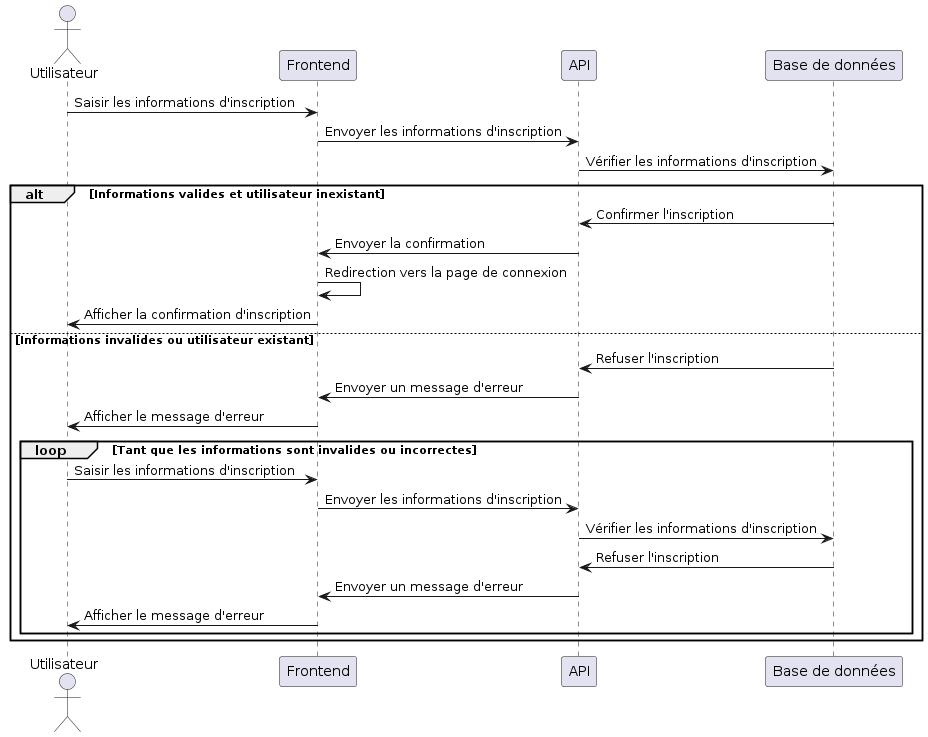
\includegraphics[width=15cm]{gfx/fig-register-seq.png}
        \caption{Diagramme de séquence pour l'inscription}.
        \label{fig:register-sequence}
    \end{figure}

    Dans ce diagramme de séquence, l'alt (alternative) montre les deux possibilités : si les identifiants sont corrects, l'utilisateur est authentifié ; sinon, un message d'erreur est affiché et l'utilisateur est invité à saisir à nouveau ses identifiants jusqu'à ce qu'ils soient corrects.

    \newpage
    \item \textbf{S’authentifier :}  Permet à un utilisateur existant de se connecter à la plateforme en fournissant ses identifiants (nom d'utilisateur et mot de passe).

    \begin{figure}[H]
        \centering
        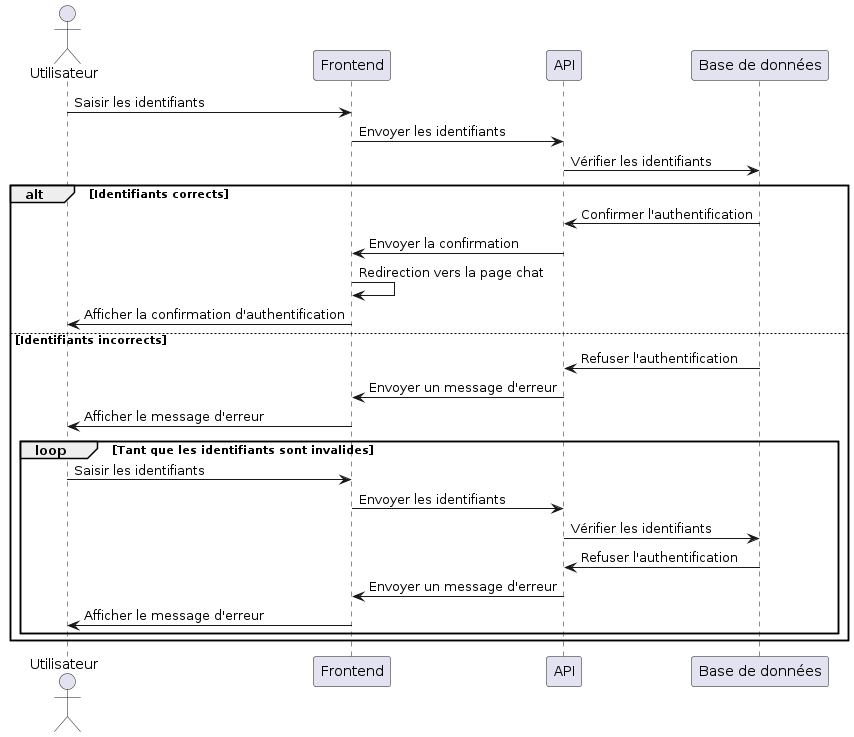
\includegraphics[width=15cm]{gfx/fig-login-seq.png}
        \caption{Diagramme de séquence pour la connexion}.
        \label{fig:login-seq}
    \end{figure}

    Dans ce diagramme de séquence, l'alt (alternative) montre les deux possibilités : si les informations sont valides et que l'utilisateur n'existe pas, l'inscription est confirmée ; sinon, un message d'erreur est affiché et l'utilisateur est invité à saisir à nouveau ses informations jusqu'à ce qu'elles soient correctes.

    \newpage
    \item \textbf{Créer un nouveau chat :} Permet à l'utilisateur de créer une nouvelle session de chat. L'utilisateur peut nommer cette session et commencer à interagir avec le chatbot.

    \begin{figure}[H]
        \centering
        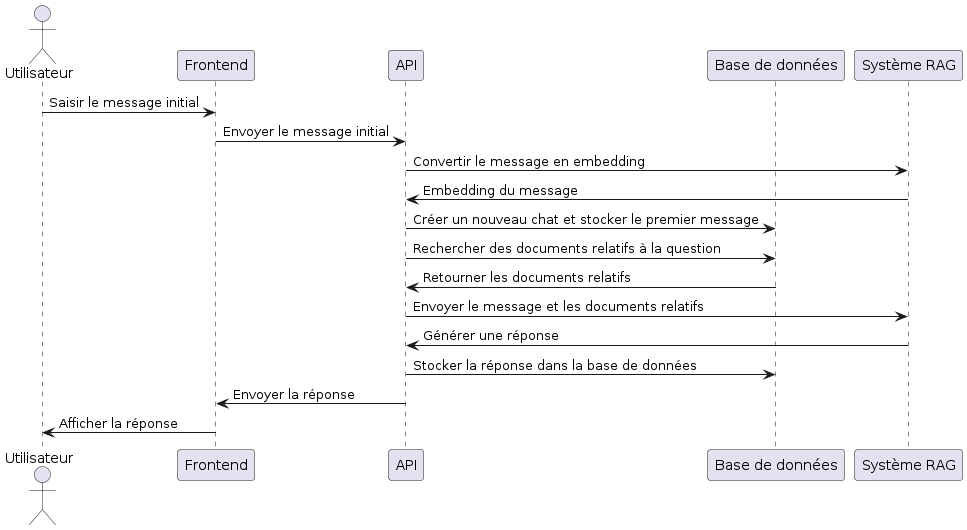
\includegraphics[width=15cm]{gfx/fig-create-chat-seq.png}
        \caption{Diagramme de séquence pour la création d'un chat}.
        \label{fig:create-chat-seq}
    \end{figure}

    \item \textbf{Envoyer un message :} Permet à l'utilisateur d'envoyer un message dans une session de chat active. Le message est traité par le système \ac{rag} pour générer une réponse appropriée.

    \begin{figure}[H]
        \centering
        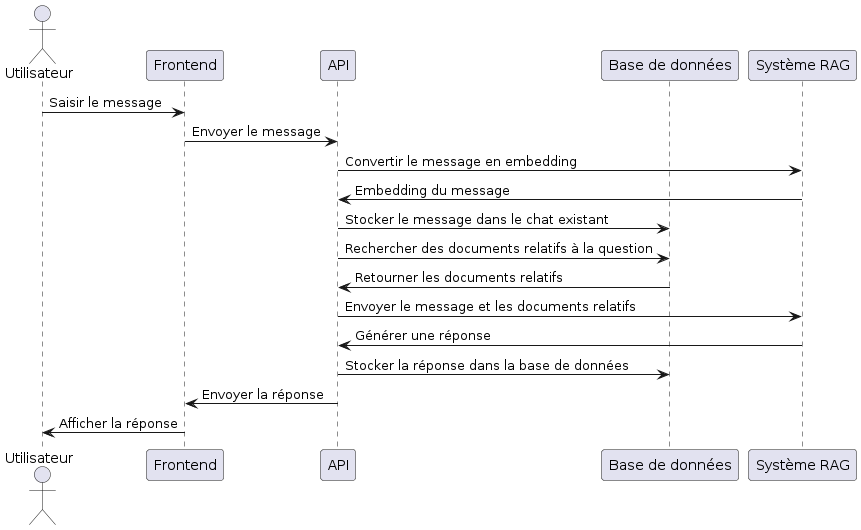
\includegraphics[width=15cm]{gfx/fig-send-message-fig.png}
        \caption{Diagramme de séquence pour l'envoie d'un message}.
        \label{fig:send-message-seq}
    \end{figure}

    \newpage
    \item \textbf{Renommer un chat :} Permet à l'utilisateur de modifier le nom d'une session de chat existante pour une meilleure organisation.

    \begin{figure}[H]
        \centering
        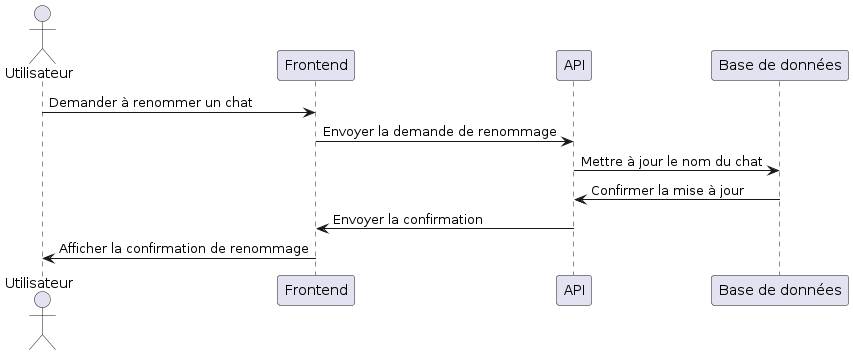
\includegraphics[width=15cm]{gfx/fig-rename-chat-seq.png}
        \caption{Diagramme de séquence pour modifier du chat}.
        \label{fig:rename-chat-seq}
    \end{figure}

    \item \textbf{Supprimer un chat :} Permet à l'utilisateur de supprimer une session de chat existante. Cette action est irréversible et supprimera toutes les données associées au chat.

    \begin{figure}[H]
        \centering
        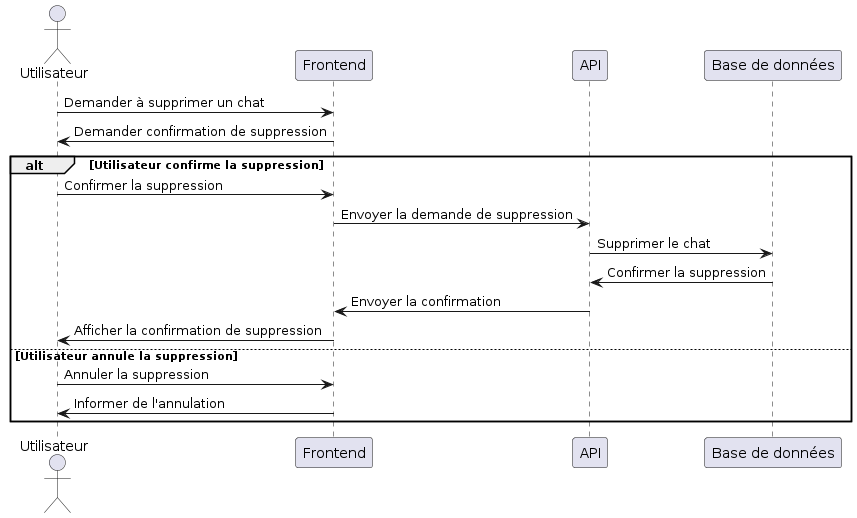
\includegraphics[width=15cm]{gfx/fig-delet-chat-seq.png}
        \caption{Diagramme de séquence pour la suppression du chat}.
        \label{fig:delete-chat-seq}
    \end{figure}

    \item \textbf{Consulter les chats :} Permet à l'utilisateur de voir la liste de toutes les sessions de chat créées. L'utilisateur peut sélectionner un chat pour le consulter ou pour effectuer d'autres actions comme renommer ou supprimer.

    \item \textbf{Choisir un chat proposé :} Permet à l'utilisateur de sélectionner un chat parmi une liste de chats proposés, basée sur des suggestions ou des chats précédemment sauvegardés.
\end{itemize}


\subsection{Le backend - API}

\begin{figure}[H]
    \centering
    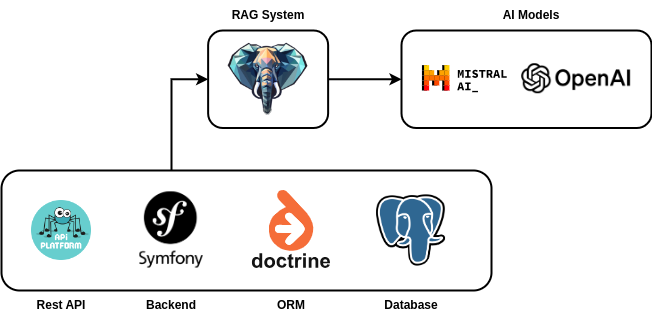
\includegraphics[width=14cm]{gfx/fig-api-architecture.png}
    \caption{Architecture du backend et services tiers}.
    \label{fig:api-architecture}
\end{figure}

L'architecture backend de notre application repose sur plusieurs technologies clés qui travaillent ensemble pour fournir une expérience utilisateur fluide et performante

\begin{itemize}
    \item \textbf{REST API :}
    API Platform \footnote{\href{https://api-platform.com/}{https://api-platform.com/}} est un framework utilisé pour créer des \ac{api} \ac{rest} robustes et bien structurées. Elle facilite la communication entre le frontend et le backend en exposant des endpoints que le frontend peut appeler pour interagir avec le système.
    
    Les requêtes \ac{http} envoyées par le frontend sont reçues par API Platform, qui les traite et les dirige vers les contrôleurs appropriés dans le backend.

    \begin{figure}[H]
        \centering
        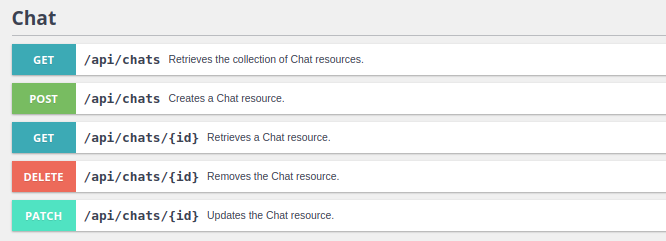
\includegraphics[width=15cm]{gfx/fig-api-doc.png}
        \caption{Documentation de l'API générer par API Platform}.
        \label{fig:api-doc}
    \end{figure}

    \item \textbf{Backend (Symfony) :}
    Symfony \footnote{\href{https://symfony.com/}{https://symfony.com/}} est le framework \acs{php} utilisé pour développer le backend de l'application. Il fournit une structure solide pour construire des applications web robustes, en facilitant la gestion des requêtes, la logique métier, et les services.
    
    Lorsque API Platform reçoit une requête, il appelle les contrôleurs Symfony qui contiennent la logique nécessaire pour traiter la requête. Symfony gère également les interactions avec le système RAG et la base de données.

    \item \textbf{ORM (Doctrine) :}
    Doctrine \footnote{\href{https://www.doctrine-project.org/}{https://www.doctrine-project.org/}} est un \ac{orm} utilisé pour interagir avec la base de données de manière abstraite. Il permet de manipuler les données en utilisant des objets \acs{php} plutôt que des requêtes \acs{sql} brutes.
    
    Les contrôleurs Symfony utilisent Doctrine pour accéder à la base de données PostgreSQL. Doctrine traduit les opérations sur les objets \acs{php} en requêtes \acs{sql} et les exécute sur la base de données.

    \item \textbf{Base de donnée (PostgreSQL) :}
    PostgreSQL est le système de gestion de base de données relationnelle utilisé pour stocker les données de l'application, y compris les utilisateurs, les messages, les chats, et les embeddings.
    
    Doctrine interagit directement avec PostgreSQL pour effectuer des opérations de lecture et d'écriture. Les données sont stockées et récupérées selon les besoins de l'application.

    \begin{figure}[H]
        \centering
        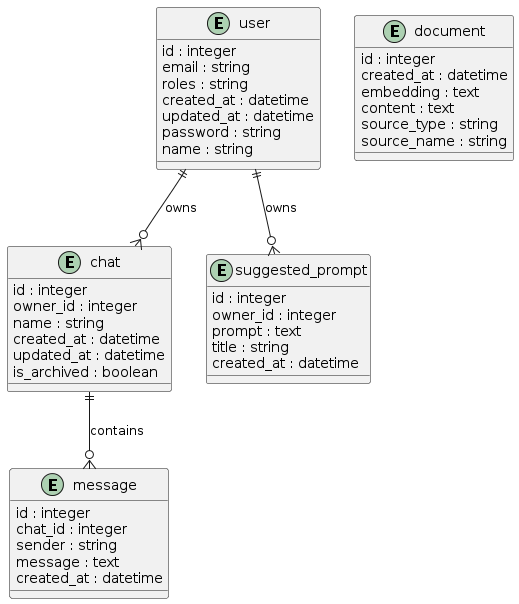
\includegraphics[width=10cm]{gfx/fig-database-schema.png}
        \caption{Diagramme relationnel d'entité}
        \label{fig:database-schema}
    \end{figure}

    \item \textbf{RAG System (LLPhant) :}
    LLPhant \footnote{\href{https://llphant.io/}{https://llphant.io/}} est un framework utilisé pour générer des réponses en utilisant des modèles d'\ac{ia}. Il combine des techniques de récupération d'informations et de génération de texte pour fournir des réponses précises et contextuelles.
    
    Lorsqu'une requête nécessite une réponse contextuelle, Symfony appelle le système \ac{rag}. Ce système utilise les embeddings stockés dans PostgreSQL pour trouver les documents pertinents, puis génère une réponse en s'appuyant sur des modèles d'\ac{ia} (comme ceux de Mistral AI \footnote{\href{https://console.mistral.ai/}{https://console.mistral.ai/}} et OpenAI \footnote{\href{https://openai.com/}{https://openai.com/}}).

    \item \textbf{Les modèles d'\ac{ia}}
    Ces modèles d'\ac{ia} sont utilisés pour convertir les questions en embeddings et générer des réponses basées sur les documents récupérés.
    
    Le système \ac{rag} envoie les questions aux modèles d'\ac{ia} pour les convertir en embeddings. Il utilise également ces modèles pour générer des réponses contextuelles basées sur les informations récupérées de la base de données.
\end{itemize}

\section{Déploiement et mis en production}
\label{ch:2:section:deploy}

\begin{figure}[H]
    \centering
    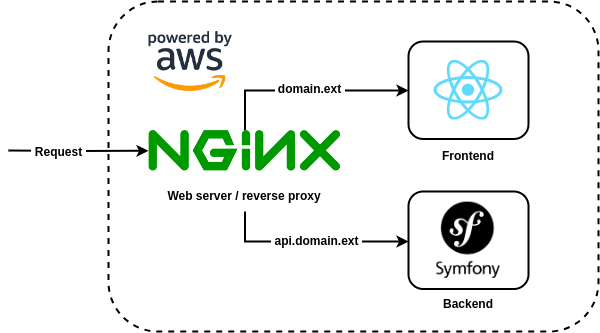
\includegraphics[width=15cm]{gfx/fig-deploy-architecture.png}
    \caption{Architecture de production}
    \label{fig:deploy-architecture}
\end{figure}

Toutes les composantes de l'application (NGINX \footnote{\href{https://nginx.org/}{https://nginx.org/}}, frontend, backend) sont déployées sur l'infrastructure AWS \footnote{\href{https://aws.amazon.com/}{https://aws.amazon.com/}}, assurant scalabilité, fiabilité et disponibilité.

NGINX, Sert de serveur web et de reverse proxy pour gérer les requêtes des utilisateurs. NGINX distribue les requêtes entre le frontend et le backend, selon le type de requête (client-side vs server-side).

\subsection{Configuration du pare-feu}

Une fois une instance (machine virtuelle) créée, nous pouvons y attacher une adresse \ac{ip} statique. Cette adresse \ac{ip} statique garantit que l'adresse attribuée à l'instance ne changera pas après un redémarrage ou une ré-initialisation de celle-ci, assurant ainsi une accessibilité constante et fiable.

Pour sécuriser notre plateforme, nous mettons en place des mesures strictes de contrôle des accès. Nous restreignons l'ouverture des ports réseau uniquement à ceux nécessaires au fonctionnement de nos services. Les ports autorisés sont :

\begin{itemize}
    \item \textbf{SSH (port 22)} : Utilisé pour les connexions sécurisées à distance, permettant aux administrateurs de gérer l'instance de manière sécurisée.
    
    \item \textbf{HTTP (port 80)} : Utilisé pour le trafic web non sécurisé, permettant aux utilisateurs d'accéder à l'application web.
    
    \item \textbf{HTTPS (port 443)} : Utilisé pour le trafic web sécurisé, garantissant que les données transmises entre l'utilisateur et le serveur sont cryptées.
    
    \item \textbf{PostgreSQL (port 5432)} : Utilisé pour les connexions à la base de données PostgreSQL, permettant aux services backend de lire et d'écrire des données de manière sécurisée.
\end{itemize}

En limitant l'accès à ces ports spécifiques, nous minimisons les risques d'attaques potentielles en réduisant la surface d'attaque disponible. Cela contribue à protéger notre infrastructure et à garantir que seuls les services nécessaires sont accessibles, tout en empêchant les accès non autorisés aux autres ports. Cette stratégie de sécurité est cruciale pour maintenir l'intégrité et la confidentialité de notre plateforme.

\begin{figure}[H]
    \centering
    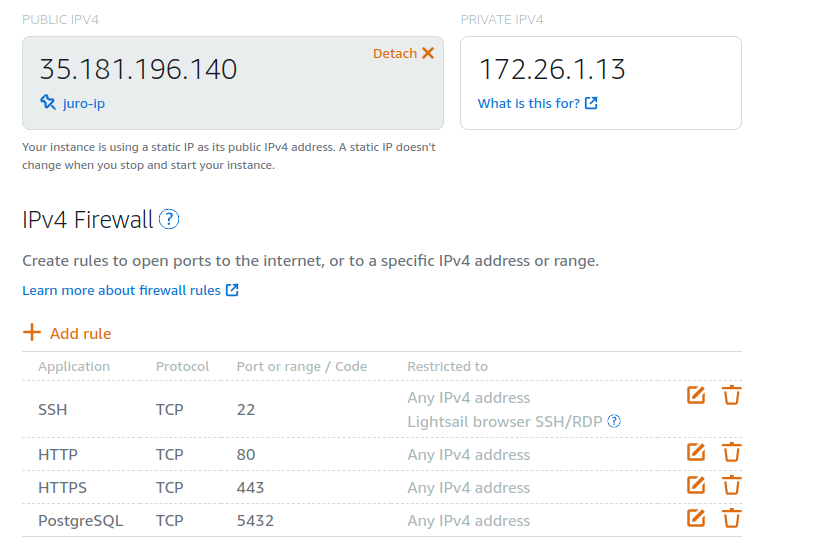
\includegraphics[width=15cm]{gfx/fig-firewall.png}
    \caption{Configuration Firewall}
    \label{fig:firewall}
\end{figure}

\subsection{Configuration du nom de domaine, DNS}

Pour la configuration \ac{dns}, nous ajoutons un enregistrement de type A pour lier le nom de domaine "juro.life" à l'adresse \ac{ip} statique de notre instance. Cet enregistrement de type A assure que toute requête dirigée vers "juro.life" est résolue en direction de l'adresse \ac{ip} associée, permettant aux utilisateurs d'accéder à notre application de manière fiable.

Afin de gérer les sous-domaines de manière efficace, nous utilisons la même adresse \ac{ip} statique. Cela signifie que nous créons des enregistrements \ac{dns} supplémentaires pour chaque sous-domaine requis, tels que "api.juro.life" et "www.juro.life", et les faisons pointer vers la même adresse \ac{ip} statique. Cette approche simplifie la gestion \ac{dns} et garantit que toutes les sous-domaines de notre domaine principal sont correctement résolus vers notre instance.

\begin{figure}[H]
    \centering
    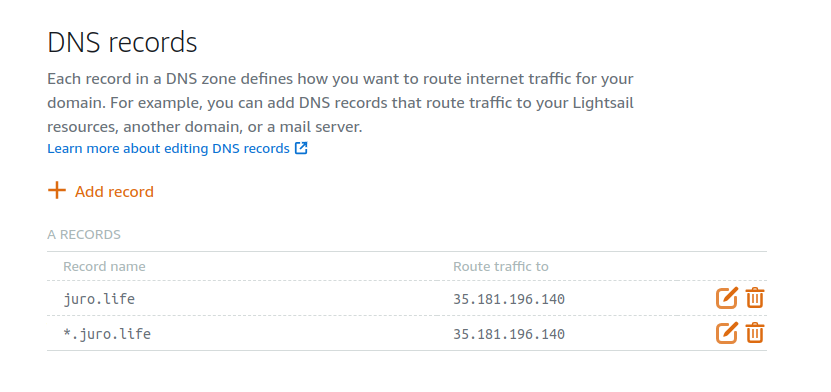
\includegraphics[width=15cm]{gfx/fig-dns-record.png}
    \caption{Configuration \acf{dns}}
    \label{fig:dns}
\end{figure}

\subsection{Configuration du reserve proxy}

Maintenant que nous avons une adresse \ac{ip} statique et un nom de domaine pointant vers cette adresse, nous pouvons configurer notre serveur pour rediriger les requêtes \ac{http} associées au domaine ou aux sous-domaines vers les applications appropriées qui tournent sur le serveur. De plus, nous mettons en place une redirection \ac{https} pour assurer que toutes les communications entre les utilisateurs et notre application sont sécurisées.

\begin{listing}[!ht]
\begin{minted}{text}
server {
    server_name api.juro.life;
    root /var/www/html/juro-api/public;
    index index.php index.html index.htm index.nginx-debian.html;

    location / {
        root /var/www/html/juro-api;
        try_files /public/$uri /assets/$uri /index.php?$query_string;
    }
}
\end{minted}
\caption{Exemple de configuration du server web}
\label{appendix:code:conf:web-nginx}
\end{listing}

Pour assurer la sécurité des communications, nous redirigeons automatiquement les requêtes \ac{http} vers \ac{https}. Voici comment configurer cette redirection dans NGINX

\begin{listing}[!ht]
\begin{minted}{text}
server {
    if ($host = api.juro.life) {
        return 301 https://$host$request_uri;
    }

    listen 80;

    server_name api.juro.life;
    return 404;
}
\end{minted}
\caption{Exemple de rédirection automatique vers HTTPS}
\label{appendix:code:conf:web-http}
\end{listing}

En configurant NGINX de cette manière, nous assurons que toutes les requêtes \ac{http} vers notre domaine et ses sous-domaines sont correctement redirigées vers les applications respectives. De plus, en forçant les redirections vers \ac{https}, nous garantissons la sécurité des communications entre les utilisateurs et notre serveur. Cette configuration robuste permet de gérer efficacement les accès à notre plateforme tout en maintenant un haut niveau de sécurité.

\section{Résumé du chapitre}

\begin{figure}[H]
    \centering
    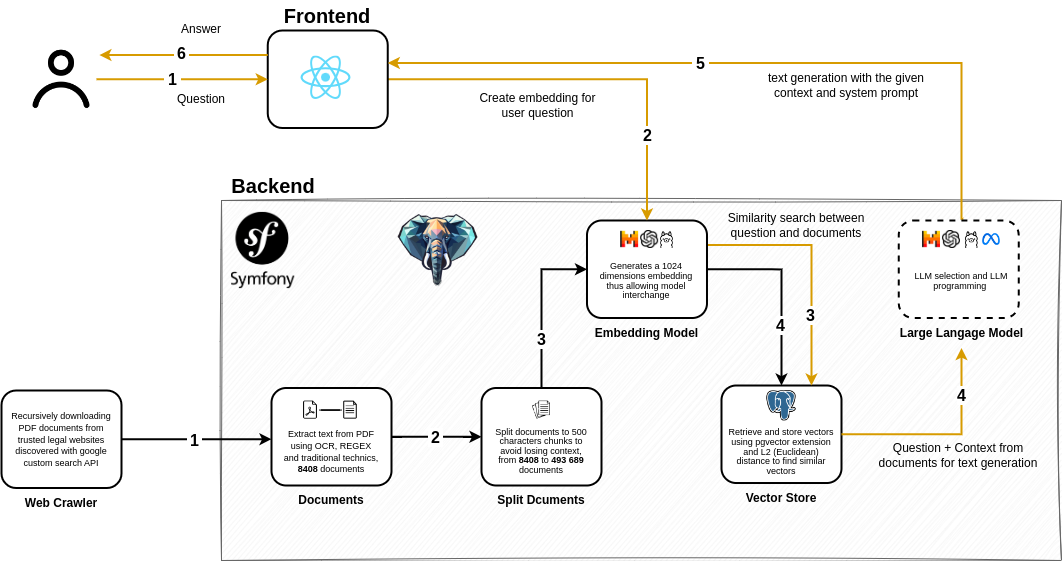
\includegraphics[width=15cm]{gfx/architecture.png}
    \caption{Achitecture}
    \label{fig:architecture-juro}
\end{figure}

Ce chapitre a fourni une vue d'ensemble complète et détaillée des différentes étapes et composantes impliquées dans la conception, le développement et le déploiement de notre chatbot juridique, mettant en évidence les choix technologiques et les stratégies d'implémentation adoptées pour créer un système performant et fiable.
